\documentclass{article}
\usepackage[utf8]{inputenc}

\title{Rapport Mystic-Tarot}
\author{Lucas.Oster }
\date{December 2020}

\usepackage{natbib}
\usepackage{graphicx}
\usepackage[english,main=french]{babel}
\begin{document}



\maketitle

\begin{figure}[!h]
\centering
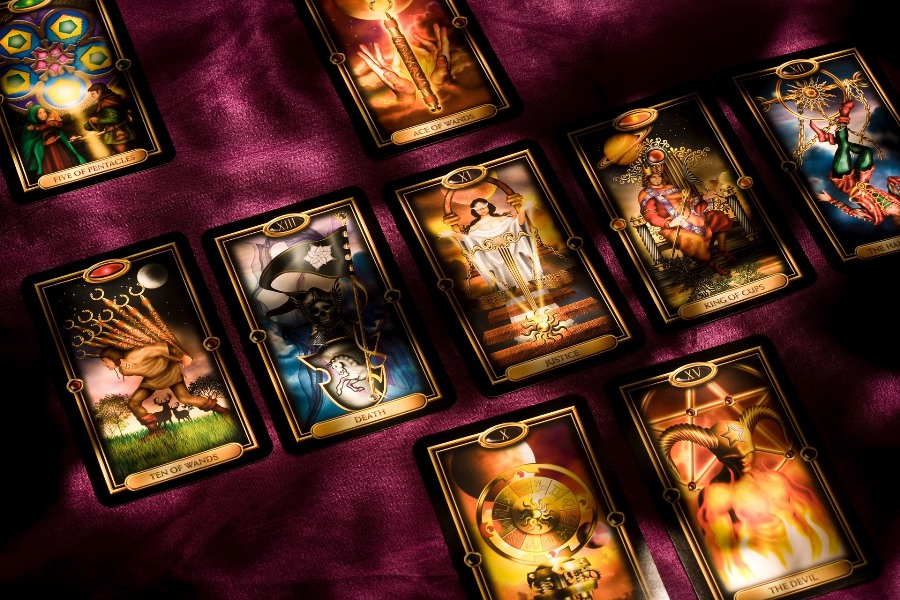
\includegraphics[scale=1]{tarot}
\caption{le tarot}
\label{fig:le tarot}
\end{figure}

\newpage

\tableofcontents
\newpage
\section{Introduction}
Le but de ce projet est de faire un programme JAVA qui permet à l'utilisateur de gérer un paquet de cartes de tarot avec une interface graphique (il peut voir le paquet, le modifier, supprimer des cartes, rechercher des cartes, ajouter des cartes, et afficher la carte selectionnée).
Toutes ces fonctionalités ont bien été implémentées.




\section{Choix architecturaux}
L'architecture MVC s'est imposée comme une évidence pour bien séparer la représentation du jeu par le modèle, de la vue et du contrôleur.
Dans cette partie nous vous présenterons donc les choix architecturaux du modèle, de la vue et du contrôleur.
\subsection{Modèle}
Dans le modèle nous avons trois classes, Carte, JeuCartesTarot et LectureEcritureSerial.

La classe Carte contient le nom, la description et l'image de la carte.
Elle permet la création d'une carte ainsi que toutes les modifications utiles.

La classe JeuCartesTarot regroupe les cartes dans une ArrayList, le choix d'une Arraylist apporte de la souplesse sur le nombre de cartes que contient le jeu et facilite la suppression et l'ajout d'une carte.
La classe JeuCartesTarot permet :

-la création d'un jeu de cartes

-la recherche d'une carte par son nom ou son numéro

-la suppression d'une carte

De plus les méthodes toString() et generationDeNeufCartes() ont étés écrites pour faciliter la tâche du développeur : on génère 9 cartes de base, on les affiche et on les sauvegarde pour tester le modèle.

La classe LectureEcritureSerial permet de sauvegarder le jeu de cartes et de lire la sauvegarde du jeu.

\subsection{Vue}
Dans la vue nous avons six classes, AfficheCartesPane, BoutonCarte, CarteUniquePanel, ConstantesCouleursFonts, FenetreTarot et PanelGauche.

La classe AfficheCartePane permet d'afficher toutes les cartes sous forme de bouton créé dans la classe BoutonCarte.
Pour permettre au contrôleur d'écouter les boutons on utilise la méthode enregistreEcouteur().

La classe BoutonCarte permet de stocker les cartes dans des boutons, en effet chaque cartes est representée par une ImageBouton, j'ai choisi de mettre les cartes directement dans des boutons pour faciliter la selection dans la classe AfficheCartesPanel d'une carte pour son affichage dans la classe CarteUniquePane.

La classe CarteUniquePanel permet d'afficher la carte selectionée et de la modifier ou la supprimer.
La méthode setCarte permet de rafraîchir l'affichage après une action sur les cartes.
Pour permettre au contrôleur d'écouter les boutons on utilise la méthode enregistreEcouteur().

La classe ConstantesCouleursFonts permet de stocker dans des variables des couleurs et des polices pour l'affichage des panels.

La classe FenetreTarot permet de rassembler tous les panels et réalise un affichage complet.

La classe PanelGauche permet d'afficher les champs pour:

-la recherche de carte par numèro ou nom 

-la création d'une carte en choissisant le nom, la description et l'image.

Pour permettre au contrôleur d'écouter les boutons on utilise la méthode enregistreEcouteur().

La barre de menu permet de quitter l'application ou de sauvegarder les modifications.

\subsection{Contrôleur}
Dans le contrôleur nous avons une classe Controleur.

Elle permet de gerer les évènements comme :

	   -les recherches
	   
	   -les suppressions
	   
	   -les modifications
	   
	   -les créations de cartes
	   
	   -l'afichage des attributs d'une carte selectionnée
	   
	   -l'ouverture d'une photo pour la création de carte
	   
	   -les actions menu (quitter et sauvegarder)


\section{Guide Utilisateur}
Dans cette partie nous montrerons comment utiliser toutes les fonctionalités des panels.

\subsection{Menu-bar}

La barre de menu permet de quitter l'application ou de sauvegarder le jeu de cartes.

\begin{figure}[!h]
\centering
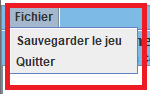
\includegraphics[scale=1]{bar_menu.png}
\caption{le barre de Menu}
\label{fig:bar_menu}
\end{figure}

\newpage
\subsection{Panel-gauche}
Ce panel sert à afficher les champs pour rechercher une carte avec son nom ou son numéro ainsi que pour créer une nouvelle carte.

\begin{figure}[!h]
\centering
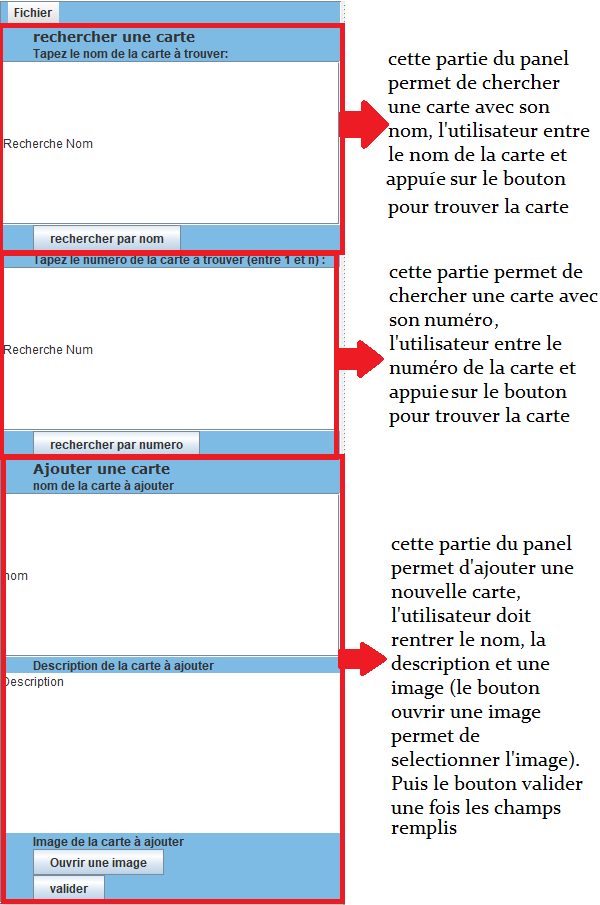
\includegraphics[scale=1]{PanelGauche2.PNG}
\caption{PanelGauche}
\label{fig:PanelGauche}
\end{figure}

\newpage
\subsection{Affiche-cartes}
Ce panel sert à afficher les cartes sous forme de bouton et de selectionner une carte.
\begin{figure}[!h]
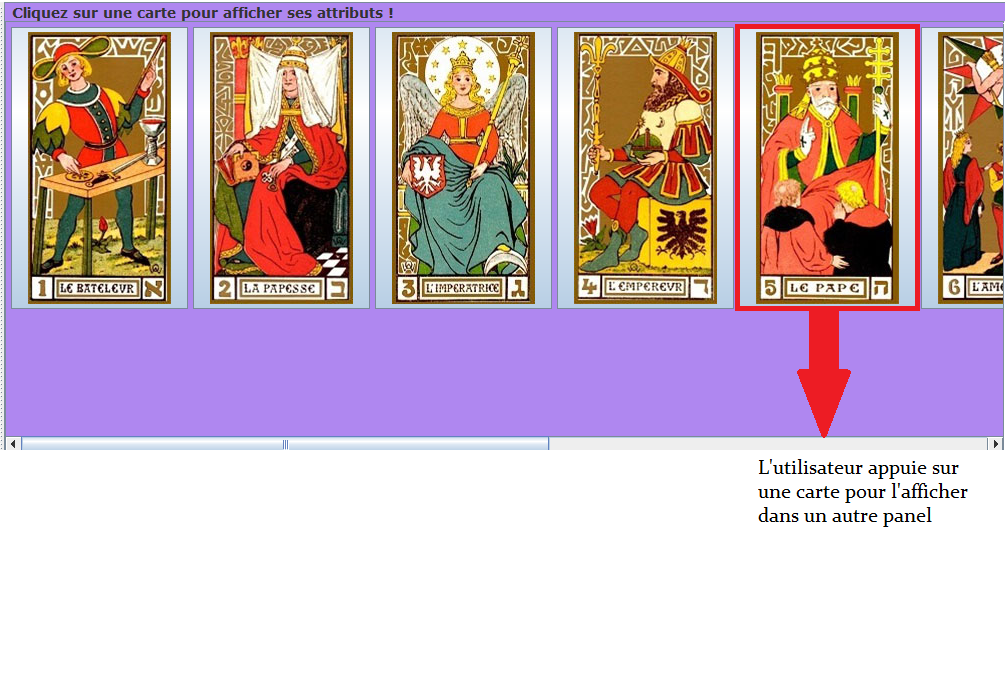
\includegraphics[scale=0.80]{AfficheCartes.PNG}
\caption{AfficheCarte}
\label{fig:AfficheCartes}
\end{figure}

\newpage
\subsection{Carte-Unique}
Ce panel sert à afficher la carte selectionnée, on peut la modifier ou la supprimer.
Au démarrage de l'application par défaut ce panel affiche la première carte du jeu.
La carte affichée est la carte séléctionée ou la carte trouver lors d'une recherche.
Lors d'une création de carte, la carte créée est affichée.

\begin{figure}[!h]

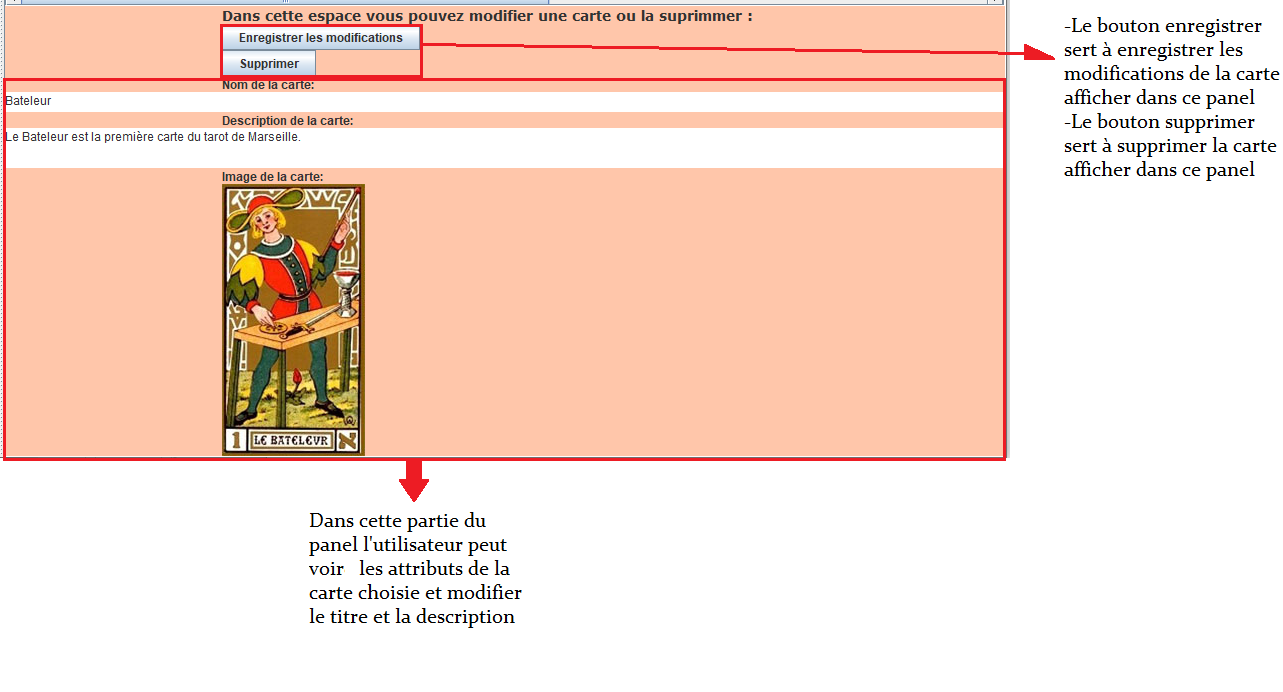
\includegraphics[scale=0.72]{CarteUnique.PNG}
\caption{CarteUnique}
\label{fig:CarteUnique}
\end{figure}

\newpage
\subsection{FenetreTarot}
Ce panel est le panel principal, il regroupe tous les autres panels pour un affichage global de l'application.

\begin{figure}[!h]
\centering
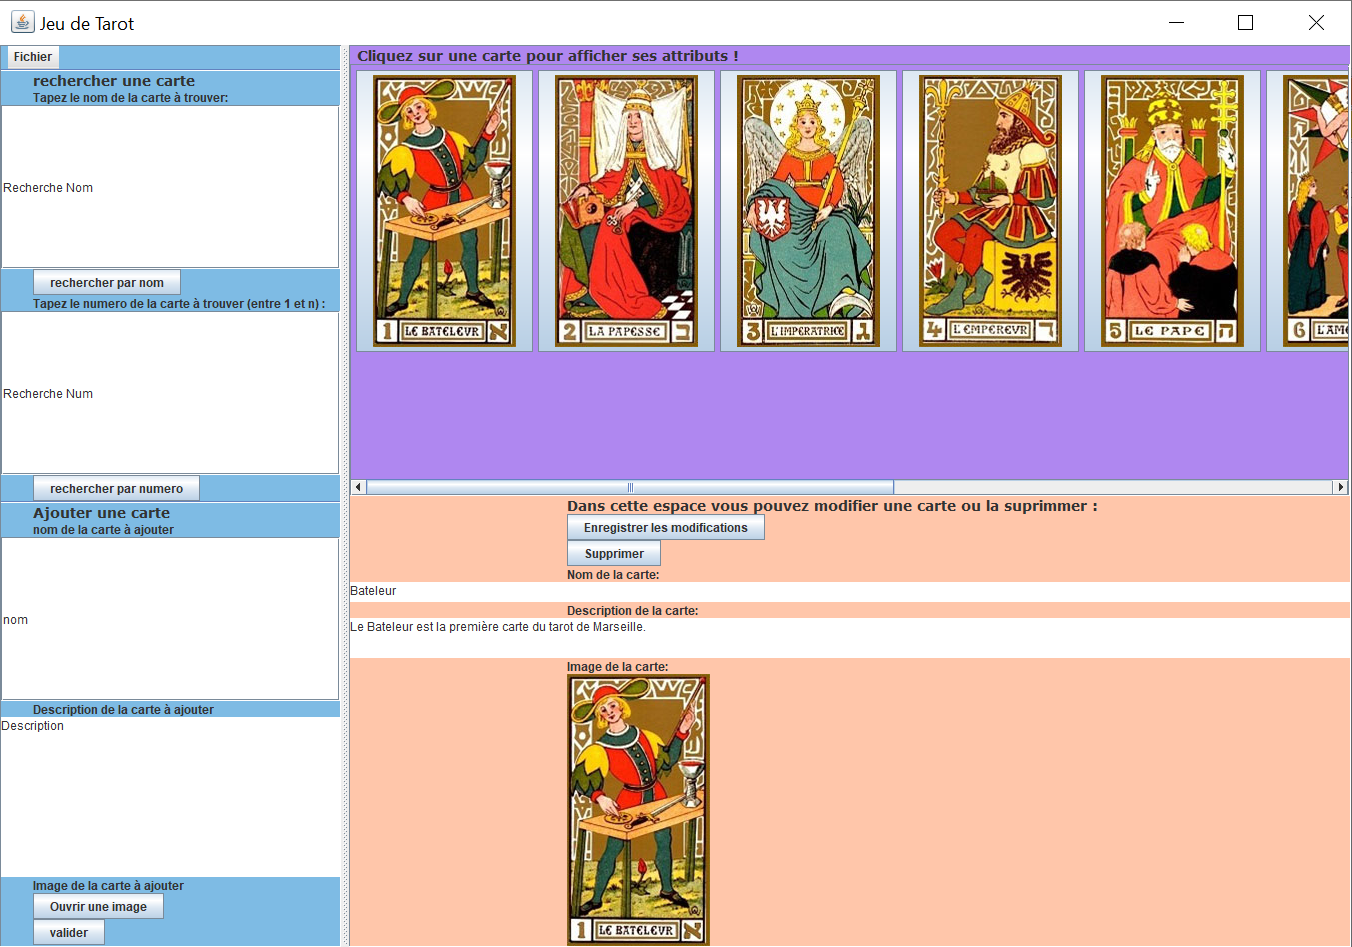
\includegraphics[scale=0.60]{FenetreTarot.PNG}
\caption{FenetreTarot}
\label{fig:FenetreTarot}
\end{figure}

\newpage
\section{Conclusion}
La réalistion de l'application MysticTarot permet bien à l'utilisateur de gérer le paquet de cartes, les fonctionalités bonus restent à implementer.

De mon point de vue, ce projet m'a été très profitable car il m'a permis de mettre en pratique la partie du cours sur la gestion de projet et les interfaces graphiques.



\end{document}
